% Progress:
% SVGs <--
%%% Some of the SVGs in the Guidelines are saved as inline SVGs! Might want to get the source files.
%%% Necessary to convert SVGs to PDF. LaTeX does not support SVGs natively and Pandoc struggles with them.
%%% Pandoc needs full path to image to work.

% Basic table creation.
% Page footer with numbered pages.
% Label for figures.
% Figured out dynamic numbering and sections.
% Figured out labels to refer to sections dynamically.

% Next:
% Table styles/borders.
% What are the deciding factors to show/hide content? (where should I look?)

% Percentage characters "%" that are meant to be printed need to be escaped like so: \%.

%% Copy and paste the code snippet below to add more content displayed conditionally (i.e., content to show if a particular value was selected for an option).
%% "OptionModelicaPath" should be replaced by the modelica path without dots of the option.
%% "Modelica.Path.Of.Selected.Value" should be replaced by the modelica path with dots of the selected value that should trigger the content to show in the document.
% \ifdefined\OptionModelicaPath
% \ifdefstring{\OptionModelicaPath}{Modelica.Path.Of.Selected.Value}{
% Text to display if the value returned by \OptionModelicaPath is equal to Modelica.Path.Of.Selected.Value.
% }{}
% \fi

\documentclass[10pt]{article}
\usepackage[letterpaper]{geometry} % Sets margins of the document based on US letter standard
\usepackage{etoolbox} % Provides \ifdefstring command.
\usepackage{svg} % Provides \includesvg command. Please note that Inkscape must be in the path.
\usepackage{titlesec} % Provides \titleformat command.

% Sets the path where SVGs are found.
% \svgpath{/Users/yves/Projects/lbnl/LBL-Linkage-Widget-v2/server/src/sequence/latex-assets/}

% If \basepath is not defined, use a fallback. Useful for editing the template outside of the backend.
\providecommand{\basepath}{/Users/yves/Projects/lbnl/LBL-Linkage-Widget-v2/server/src/sequence}

% Formats title
% https://en.wikibooks.org/wiki/LaTeX/Title_Creation
\title{Control Sequence}
\author{}
\date{}

% https://latex-programming.fandom.com/wiki/LaTeX_environment
\begin{document}

\maketitle

% Adds a page break.
% http://www.personal.ceu.hu/tex/breaking.htm
\newpage

% https://overleaf.com/learn/latex/Sections_and_chapters#Document_sectioning
% https://en.wikibooks.org/wiki/LaTeX/Labels_and_Cross-referencing
\section{SETPOINTS, DESIGN and FIELD DETERMINED}
\subsection{Information Provided by Designer}

\subsubsection{VAV Box Design Information}
\paragraph{VAV Cooling-Only Terminal Unit} \label{vav_cooling_only_terminal_unit}

\section{SEQUENCES OF OPERATIONS}

\subsection{Generic Ventilation Zones} \label{generic_ventilation_zones}
\subsection{Generic Thermal Zones} \label{generic_thermal_zones}

\subsection{VAV Terminal Unit—Cooling Only}
\subsubsection{See “Generic Thermal Zones” (Section \ref{generic_thermal_zones}) for setpoints, loops, control modes, alarms, etc.}
\subsubsection{See “Generic Ventilation Zones” (Section \ref{generic_ventilation_zones}) for calculation of zone minimum outdoor airflow.}

CO2 DCV for cooling-only zones can lead to overcooling due to the faster rise in CO2 levels from people in the room versus the increase in cooling loads from people. Including heat in all zones with CO2 DCV is therefore recommended. 

\subsubsection{See Section \ref{vav_cooling_only_terminal_unit} for zone minimum airflow setpoint Vmin, zone maximum cooling airflow setpoint Vcool-max, and zone maximum heating airflow setpoint Vheat-max.}

If the minimum ventilation rate is more than 25\% or so of the cooling maximum, or DCV is used, a reheat box is recommended to avoid overcooling. DCV logic is not provided for cooling-only boxes, because doing so results in periods of overcooling, as the CO2 levels due to occupants rises much faster than the cooling load due to occupants because of thermal mass.

Cooling-only terminal units can provide heating only when the AHU supply air temperature is more than 3°C (5°F) above the room temperature.

\subsubsection{Active endpoints used in the control logic depicted in Figure \ref{figure:control_logic} shall vary depending on the mode of the Zone Group the zone is a part of (see Table \ref{figure:zone_group_mode}).}

\label{figure:zone_group_mode}
% Inserts a table.
\begin{center}
Table \ref{figure:zone_group_mode} Endpoints as a Function of Zone Group Mode 
\end{center}
%
% https://es.overleaf.com/learn/latex/Tables
\begin{tabular}{ c|c|c|c|c|c|c } 
 \hline
 Endpoint & Occupied & Cooldown & Setup & Warmup & Setback & Unoccupied \\ 
 \hline
 Cooling maximum & Vcool-max & Vcool-max & Vcool-max & 0 & 0 & 0 \\ 
 \hline
 Minimum & Vmin* & 0 & 0 & 0 & 0 & 0 \\ 
 \hline
 Heating maximum & Vheat-max & 0 & 0 & Vcool-max & Vcool-max & 0 \\ 
 \hline
\end{tabular}

\subsubsection{Control logic is depicted schematically in Figure \ref{figure:control_logic} and described in the following subsections.} \label{figure:control_logic}

% Inserts PDF image
\begin{figure}[h]
  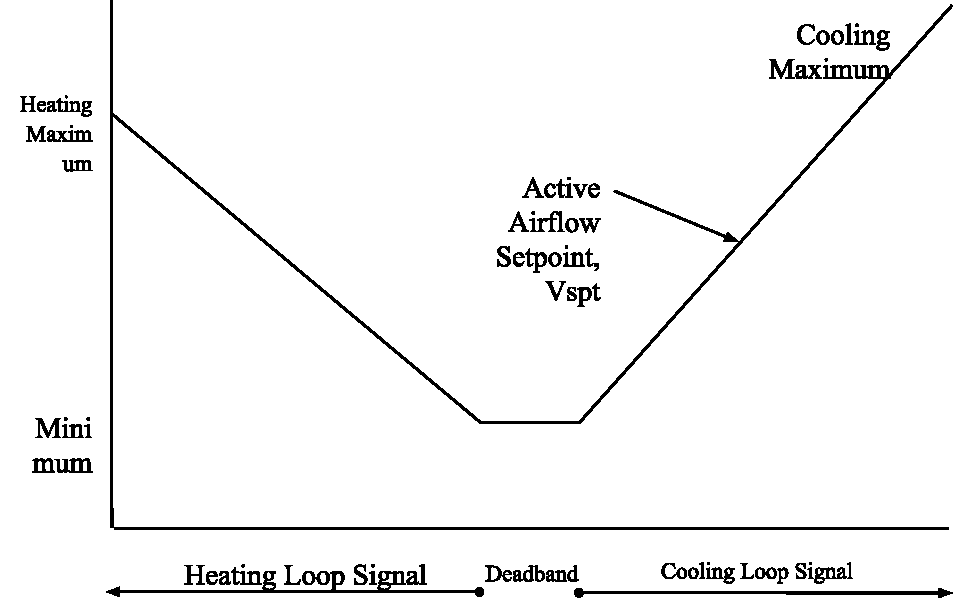
\includegraphics{\basepath/svg-inkscape/control-logic_svg-tex.pdf}
%  \includesvg{control-logic}
\end{figure}

% Inserts PNG
\begin{figure}[h]
  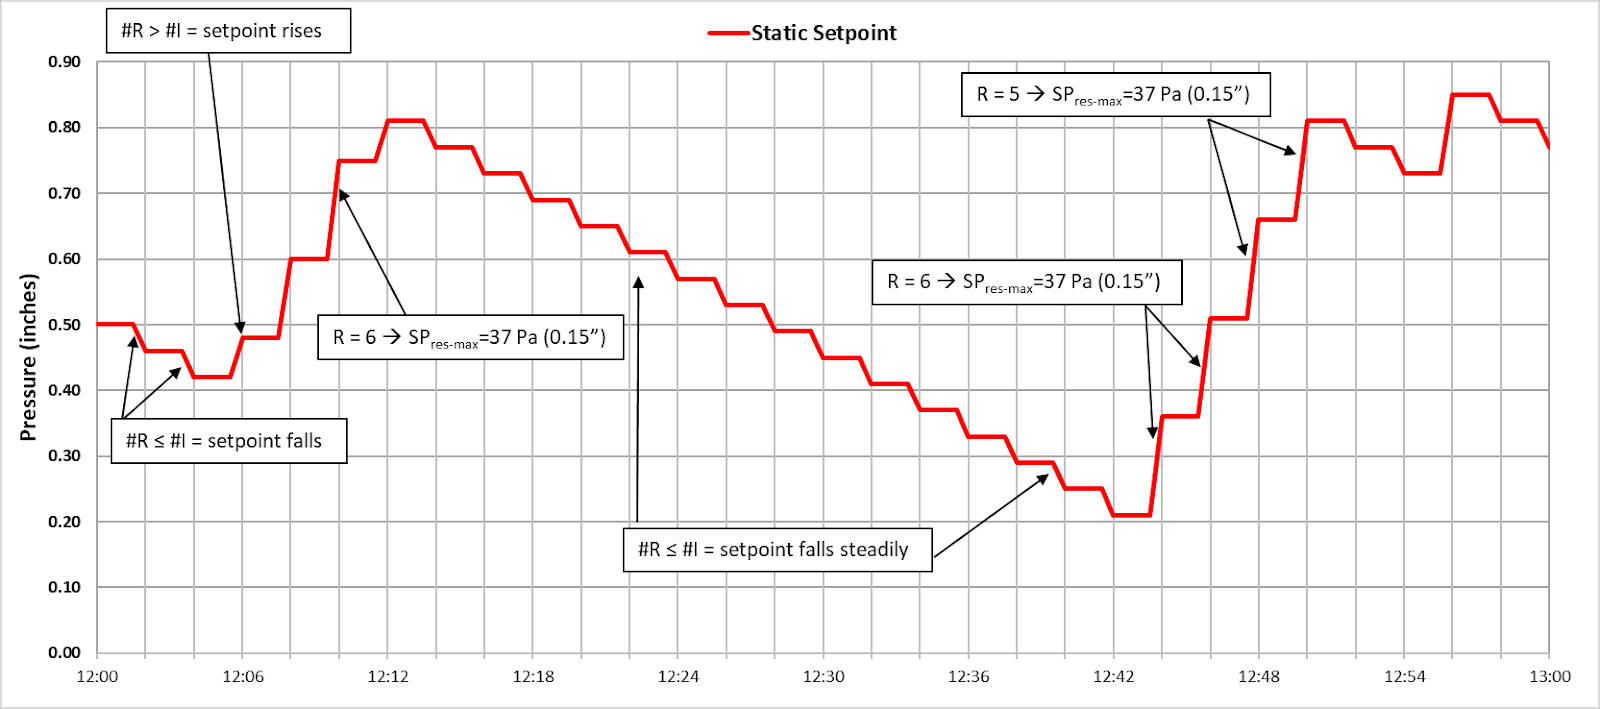
\includegraphics{\basepath/latex-assets/image6.png}
\end{figure}

\ifdefined\BuildingsTemplatesAirHandlersFansInterfacesPartialAirHandlertypFanRet
\ifdefstring{\BuildingsTemplatesAirHandlersFansInterfacesPartialAirHandlertypFanRet}{Buildings.Templates.Components.Types.Fan.SingleConstant}{
Type of return fan: Single fan - Constant speed
}{}
\fi

\end{document}
